%----------------------------------------------------------------------
\chapter*{Overview}\label{ch:overview}
\addcontentsline{toc}{chapter}{Overview}
%----------------------------------------------------------------------

\section*{Laboratory kit components}
\addcontentsline{toc}{section}{Laboratory kit components}

The laboratory kit includes:
\begin{itemize}
\item	An STM32F407 computer board, which emulates an on-board computer system (OBC).
\item	A USB A / mini USB cable which is used to connect the OBC board to the development station hosted on the student PC.
\item	A USB / UART interface cable which is used to provide a serial line link between the OBC board and the ground station software running on the student PC.
\end{itemize}

Figure~\ref{fig:kit} shows the components of the laboratory kit and the connections to the student PC.

\begin{figure}[h]
            \centering{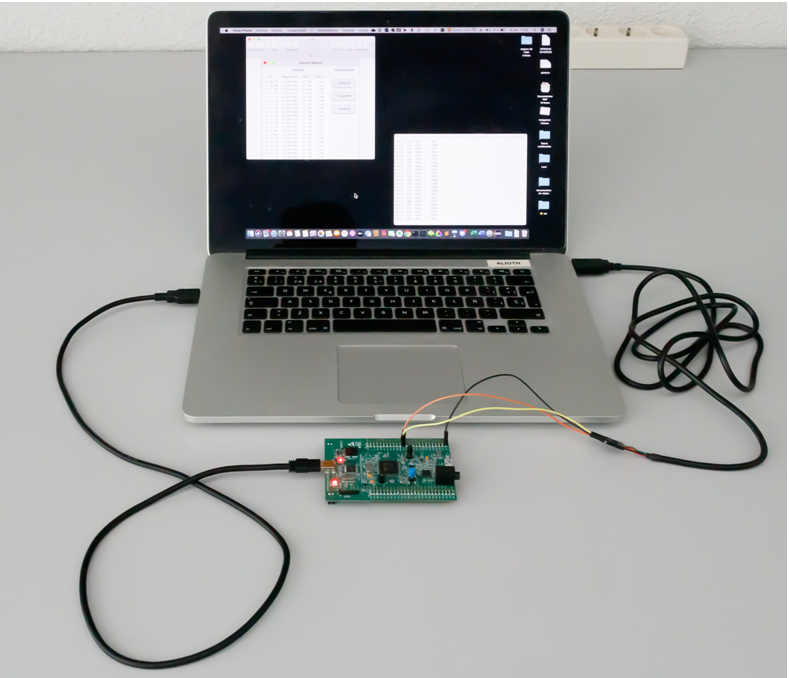
\includegraphics[width=.6\textwidth,keepaspectratio]{laboratory_kit.png}}
            \caption{Laboratory kit.}
            \label{fig:kit}
\end{figure}

\section*{Architecture of the laboratory platform}
\addcontentsline{toc}{section}{Architecture of the laboratory platform}

The components of the laboratory kit are used to emulate a simplified version of a satellite on-board software system. Figure~\ref{fig:architecture} shows the architecture of the laboratory system.

\begin{figure}[h]
            \centering{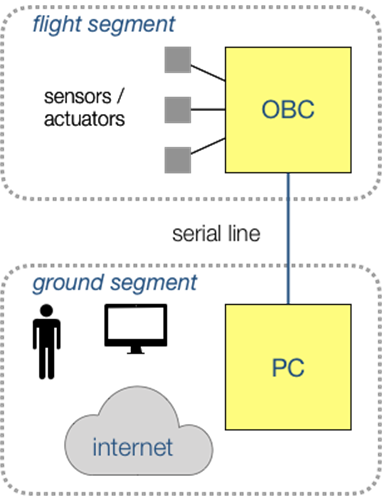
\includegraphics[width=0.35\textwidth,keepaspectratio]{architecture.png}}
            \caption{Architecture of the laboratory system.}
            \label{fig:architecture}
\end{figure}

The system consists of a flight segment, implemented on the laboratory computer board, and a ground system, implemented on the student PC. The communication between both segments is carried out by means of a serial line, simulating the radio link of a real satellite mission.
The student work is centered on programming the computer board. The ground station software will be provided by the teachers.

\section*{Computer board and connections}
\addcontentsline{toc}{section}{Computer board and connections}

The STM32F407 board is used as a low-cost replacement for a satellite on-board computer (OBC). The board features a 32-bit ARM Cortex-M4 microcomputer, 192 KB RAM, 1 MB Flash memory and a number of other devices.

Figure~\ref{fig:board} shows an overall view of the computer board.

\begin{figure}[h]
            \centering{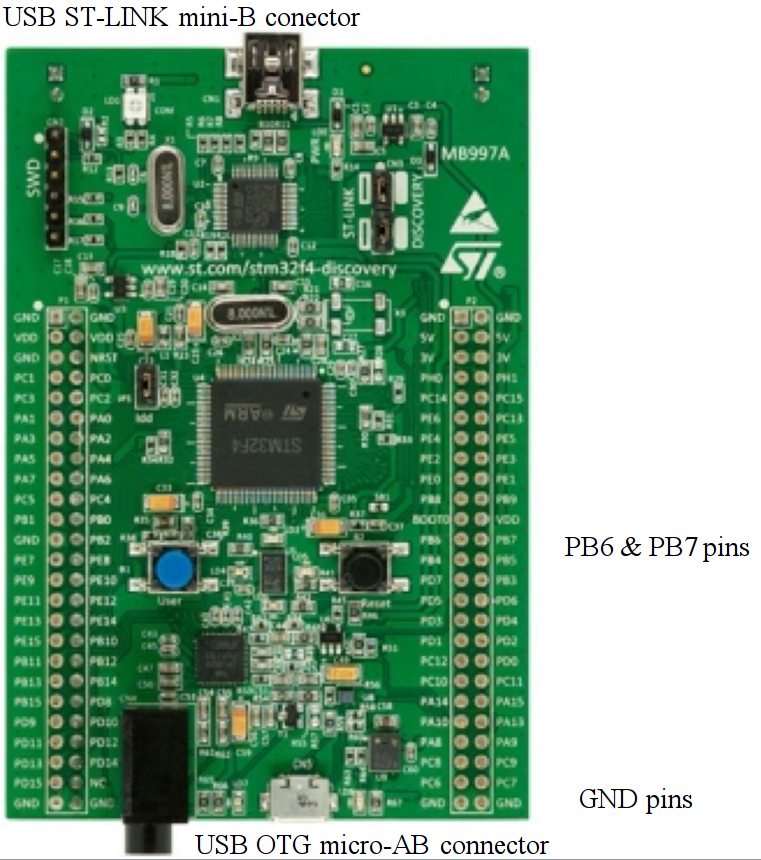
\includegraphics[height=11cm,keepaspectratio]{board.png}}
            \caption{Computer board.}
            \label{fig:board}
\end{figure}

The main elements that will be used in the laboratory are:
\begin{itemize}
\item	USB ST-LINK connector, which is linked to a PC with a mini USB-USB A cable. This connection is used for the following functions:
\begin{itemize}
\item	power supply to the board (5 V)
\item	program loading and debugging from host
\end{itemize}
\item	GPIO pins PB6, PB7 and GND. GPIO (General Purpose Input-Output) is a standard interface for connecting external devices. These GPIO pins are used in the laboratory to connect a serial line to a USB port on a PC, emulating the connection to the on-board radio equipment in a satellite.
\item	Temperature and voltage sensors. These sensors are part of the STM32 microcomputer chip, and can be read using internal registers in the MCU. They are used in the laboratory to emulate the housekeeping 
\end{itemize}
